\documentclass[12pt,a4paper]{report}
\usepackage[hmargin=3cm,vmargin=3cm]{geometry}
\usepackage{graphicx}
\usepackage{wrapfig}
\usepackage{caption}
\usepackage{array}
\usepackage{listings}
\usepackage{color}
\usepackage{hyperref}
\hypersetup{
	colorlinks=true, % make the links colored
	linkcolor=blue, % color TOC links in blue
	urlcolor=cyan, % color URLs in red
	linktoc=all % 'all' will create links for everything in the TOC
}
\graphicspath{{images/}}

\begin{document}

\begin{figure}
\centering

\includegraphics[width = 0.3\textwidth]{iit}
\hspace{1cm}

\includegraphics[width = 0.4\textwidth]{fossee-logo.png}
\end{figure}

\title{\textbf{\textbf{Summer Fellowship Report}}\vspace{4mm} \\\small On \\\vspace{4mm} \textbf{\large Title}\\ \vspace{4mm}\small Submitted by\\  \vspace{4mm}  \large \textbf{Ashutosh Gangwar}\\ \vspace{1mm} B.Tech (Computer Science and Engineering)\\ MIET, Meerut\\ \vspace{4mm} \large \textbf{Mudit Joshi}\\ \vspace{1mm} B.Tech (Computer Science and Engineering)\\ PDPM IIITDM, Jabalpur\\ \vspace{4mm} \small Under the guidance of \\ \vspace{4mm}
	\large \textbf{Prof.Kannan M. Moudgalya} \vspace{1mm}\\ Chemical Engineering Department  \vspace{1mm} \\IIT Bombay
}

\maketitle


\newpage
\title{\textbf{\textbf{\LARGE 
\begin{flushleft}
\textbf{Acknowledgment}
\end{flushleft}
}}}
\begin{flushleft}
	The fellowship opportunity we had with FOSSEE Team was a great chance for learning and professional development. Therefore, we consider ourselves as very lucky as we were provided with an opportunity to be a part of it. We are also grateful for having a chance to meet so many wonderful people and professionals who led me though this internship period.
	
	Bearing in mind previous I am using this opportunity to express my deepest gratitude and special thanks to the MD of [Company name] who in spite of being extraordinarily busy with her/his duties, took time out to hear, guide and keep me on the correct path and allowing me to carry out my project at their esteemed organization and extending during the training.
	
	I express my deepest thanks to [Name Surname], [Position in the Company] for taking part in useful decision \& giving necessary advices and guidance and arranged all facilities to make life easier. I choose this moment to acknowledge his/her contribution gratefully.
	
	It is my radiant sentiment to place on record my best regards, deepest sense of gratitude to Mr./Ms. [Name Surname], [Position in the Company], Mr./Ms. [Name Surname], [Position in the Company], Mr./Ms. [Name Surname], [Position in the Company] and Mr./Ms. [Name Surname], [Position in the Company] for their careful and precious guidance which were extremely valuable for my study both theoretically and practically.
	
	I perceive as this opportunity as a big milestone in my career development. I will strive to use gained skills and knowledge in the best possible way, and I will continue to work on their improvement, in order to attain desired career objectives. Hope to continue cooperation with all of you in the future

\end{flushleft}

\listoffigures
\tableofcontents

\chapter{\textbf{Introduction}}
FOSSEE (Free and Open Source Software in Education) project promotes the use of FOSS tools to improve the quality of education in our country. They aim to reduce dependency on proprietary software in educational institutions. They encourage the use of FOSS tools through various activities to ensure commercial software is replaced by equivalent FOSS tools. They also develop new FOSS tools and upgrade existing tools to meet requirements in academia and research. 
Incorporated to FOSSEE program, this fellowship's main aim is to introduce students to the FOSS in various engineering fields and to become a part of this big community.
\\\\
We were selected for this fellowship on the basic of screen task submitted by us. There we got opportunity to work on some of the major open source electronic simulation softwares and are introduced to the Technology Stack they are build on. These technologies include C/C++ Programming, Python, Wxwidget, WxPython, PyQt4,etc. 
\\\\
At the beginning of the fellowship we formulated several learning goals, which we want to achieve:
\begin{itemize}
	\item To understand the functioning and working conditions of a government organisation
	\item To see what it is like to work in a professional environment
	\item To see if this kind of work is a possibility for our future career
	\item To use our knowledge and skills and to further increase them
	\item To learn about organising of a open source project
	\item To enhance our communication skills
	\item To build a professional and social network
\end{itemize}
This report is a short description of our 48 days fellowship under FOSSEE. This report contains our activities that have contributed to achieve a number of our stated goals. Following is the description of the softwares we worked on and changes we have done in them, concluding with the experience we gained.
\section{KiCad}
\href{http://kicad-pcb.org/}{KiCad} is a free software suite for electronic design automation (EDA). It facilitates the design of schematics for electronic circuits and their conversion to PCB designs. KiCad was originally developed by Jean-Pierre Charras. It features an integrated environment for schematic capture and PCB layout design. Tools exist within the package to create a bill of materials, artwork, Gerber files, and 3D views of the PCB and its components.
\\
The Kicad suit has 5 main parts: 
\begin{itemize}
	\itemsep0em 
	\item KiCad – the project manager.
	\item Eeschema – the schematic capture editor.
	\item Pcbnew – the PCB layout program. It also has a 3D view.
	\item GerbView – the Gerber viewer.
	\item Bitmap2Component – tool to convert images to footprints for PCB artwork.
\end{itemize}

\begin{figure}[h]
	\centering
	
\includegraphics[scale=0.3]{KiCad-Logo}
	\caption{Kicad Logo}
	\vspace{5mm}
	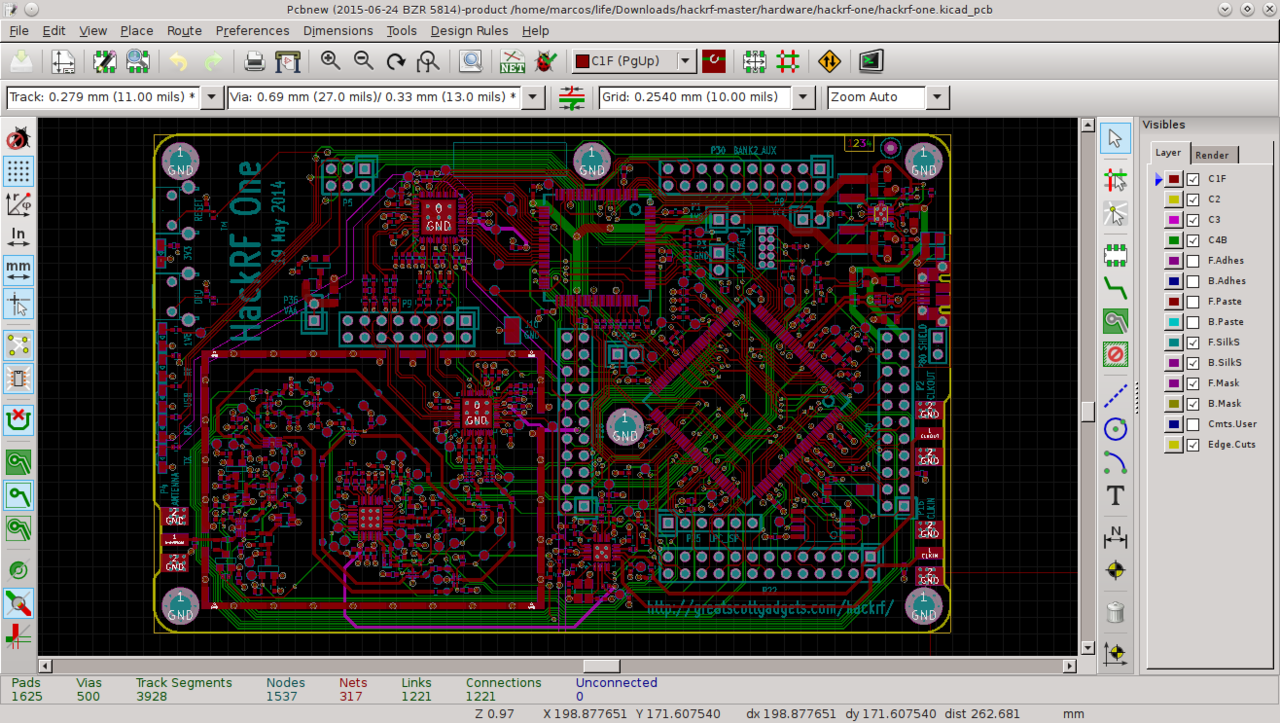
\includegraphics[width=\textwidth]{KiCad}
	\caption{Kicad PcbNew OpenGL}
\end{figure}
\vspace{5mm}

\section{eSim}
\href{https://esim.fossee.in/}{eSim} (previously known as Oscad / FreeEDA) is an open source EDA tool for circuit design, simulation, analysis and PCB design. It is an integrated tool built using open source software such as \href{http://www.kicad-pcb.org}{KiCad} and \href{http://ngspice.sourceforge.net/}{NgSpice}.eSim is released under GPL.
\\
eSim offers similar capabilities and ease of use as any equivalent proprietary software for schematic creation, simulation and PCB design, without having to pay a huge amount of money to procure licenses. Hence it can be an affordable alternative to educational institutions and SMEs. It can serve as an alternative to commercially available/ licensed software tools like OrCAD, Xpedition and HSPICE.
The eSim suit Includes: 
\begin{itemize}
	\itemsep0em 
	\item KiCad  the complete KiCad suit.
	\item KiCadtoNgSpice - Generate Ngspice netlist.
	\item NgSpice Simulation - Simulate Circuit using NgSpice backend
	\item Model Editor
	\item Subcircuit Editor - Design subcircuit fro IC's 
	\item NGHDL - Convert VHDL to Ngspice
	\item Modelica Converter - Convert Modelica files to Schematic
	\item Modelica Optimization
\end{itemize}

\begin{figure}[h]
	\centering
	
\includegraphics[scale=0.2]{eSim-logo}
	\caption{eSim Logo}
	\vspace{5mm}
	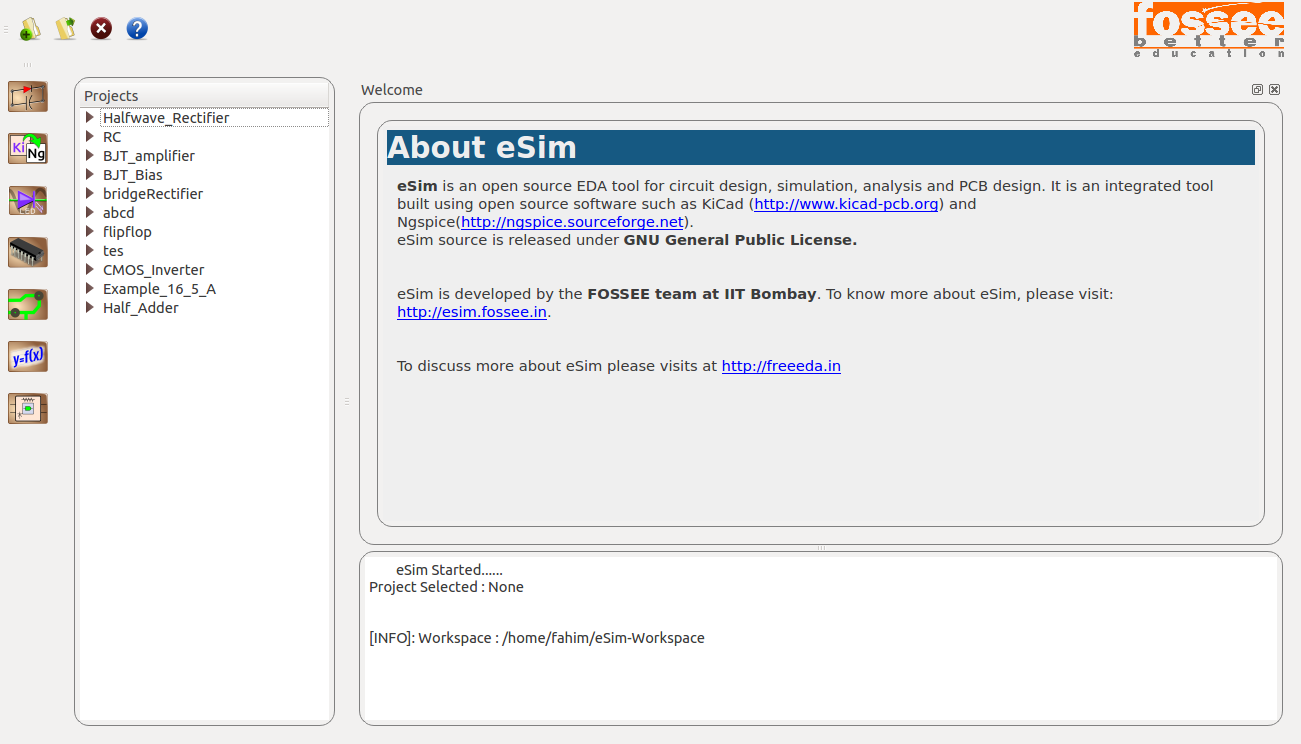
\includegraphics[width=11cm]{eSim}
	\caption{eSim Main Window}
\end{figure}


\section{ngSpice}
Ngspice is a mixed-level/mixed-signal circuit simulator. It is the open-source successor of Spice3f5. A small group of maintainers and the community of motivated users contribute to the ngspice project by providing new features, enhancements and bug fixes.

Ngspice is based on three free-software packages: Spice3f5, Xspice and Cider1b1:
\begin{itemize}
	\itemsep0em
	\item SPICE is the origin of all electronic circuit simulators, its successors are widely used in the electronics community.
	\item Xspice is an extension to Spice3 that provides additional C language code models to support analog behavioral modeling and co-simulation of digital components through a fast event-driven algorithm.
	\item Cider adds a numerical device simulator to ngspice. It couples the circuit-level simulator to the device simulator to provide enhanced simulation accuracy (at the expense of increased simulation time). Critical devices can be described with their technology parameters (numerical models), all others may use the original ngspice compact models.
\end{itemize}

Ngspice is, anyway, more than the simple sum of the packages above, as many people are contributing to the project with their experience, their bug fixes and their improvements giving ngspice additional features and improved robustness.

\begin{figure}[h]
	\centering
	
\includegraphics[scale=0.5]{ngspice-logo}
	\caption{NgSpice Logo}
	\vspace{5mm}
	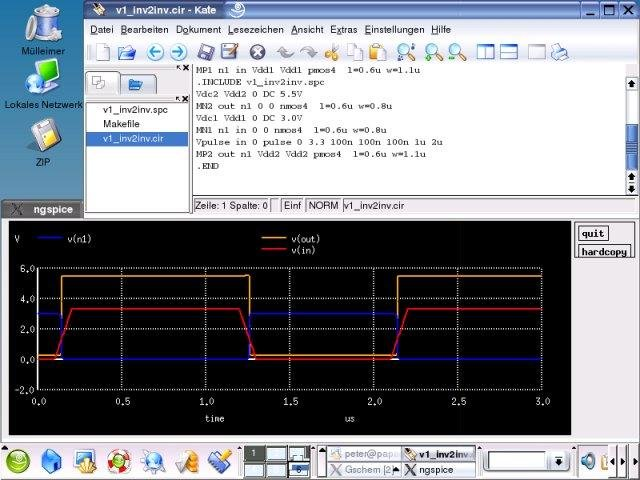
\includegraphics[height=7cm]{ngspice}
	\caption{ngSpice on KDE(Linux)}
\end{figure}


\chapter{\textbf{KiCad Nightly Build (v5)}}
\section{Build Process}
Kicad relies on various build tools and library dependencies for 
\subsection{Build Tools}
\subsubsection{\href{https://cmake.org/}{Cmake}}
Kicad uses Cmake to generate native makefiles for various platforms.
\subsubsection{\href{http://www.swig.org/}{SWIG}}
SWIG is used to generate the Python scripting language extensions for KiCad. SWIG is not required if you are not going to build the KiCad scripting extension.
\subsection{Library Dependencies}
\subsubsection{\href{https://www.wxwidgets.org/}{wxWidgets}}
wxWidgets is the graphical user interface (GUI) library used by KiCad. The current minimum version is 3.0.0. However, 3.0.2 should be used whenever possible as there are some known bugs in prior versions that can cause problems on some platforms.
\subsubsection{\href{http://www.boost.org/}{Boost C++ Libraries}}
The Boost C++ library is required only if you intend to build KiCad with the system installed version of Boost instead of the default internally built version. If you use the system installed version of Boost, version 1.56 or greater is required.
\subsubsection{\href{http://glew.sourceforge.net/}{OpenGL Extension Wrangler}}
The OpenGL Extension Wrangler is an OpenGL helper library used by the KiCad graphics abstraction library and is always required to build KiCad.
\subsubsection{\href{http://glm.g-truc.net/}{OpenGL Mathematics Library}}
The OpenGL Mathematics Library is an OpenGL helper library used by the KiCad graphics abstraction library and is always required to build KiCad.
\subsubsection{\href{https://www.opengl.org/resources/libraries/glut/}{OpenGL Utility Toolkit}}
The OpenGL Utility Toolkit is an OpenGL helper library used by the KiCad graphics abstraction library [GAL] and is always required to build KiCad.
\subsubsection{\href{http://cairographics.org/}{Cairo 2D Graphics Library}}
The Cairo 2D graphics library is used as a fallback rendering canvas when OpenGL is not available and is always required to build KiCad.
\subsubsection{\href{http://www.python.org/}{Python}}
The Python programming language is used to provide scripting support to KiCad. It needs to be installed unless the KiCad scripting build configuration option is disabled.
\subsubsection{\href{http://wxpython.org/}{wxPython}}
The wxPython library is used to provide a scripting console for Pcbnew. It needs to be installed unless the wxPython scripting build configuration option is disabled.
\subsubsection{\href{https://github.com/tpaviot/oce}{OpenCascade Community Edition}}
The OpenCascade Community Edition is used to provide support for loading and saving 3D model file formats such as STEP.
\subsubsection{\href{https://ngspice.sourceforge.net/}{ngSpice}}
The Ngspice library is used to provide Spice simulation support in the schematic editor.
\subsection{Building on Linux}
To build Kicad from source, first Cmake is used to generate the makefile for target platform\\
\begin{verbatim}
    cd <kicad source mirror>
    mkdir -p build/debug
    cmake -DCMAKE_BUILD_TYPE=Release ../../
\end{verbatim}
Once Cmake finishes generating makefile, run\\
\begin{verbatim}
    make
    sudo make install
\end{verbatim}
By default, Kicad is installed on system root in Linux. Installation path can be changed by using following while generating makefile using Cmake\\
\begin{verbatim}
    cmake ... -DCMAKE_INSTALL_PREFIX=<desired path> ...
\end{verbatim}
\section{Bug : Autoplot PDF when saving projects}
This Bug : \verb!#! 1636549 is a feature addition in Kicad which is requested by a user of Kicad. It is somtime necesary to have the schematic in a handy format (like pdf) which can be easily accesed by other non-electric background people. So the requirement is to automatically plot the schematic in PDF format whenever the user saves the schematic, as the default plot method is time consuming.
\vspace{3mm}
\\
Bug Link : \url{https://bugs.launchpad.net/kicad/+bug/1636549}
\\
\\
Patch Link : \url{https://launchpadlibrarian.net/375310564/0001-Eeschema-Adding-Autoplot-PDF-when-saving-project.patch}
\begin{figure}[h]
	\centering
	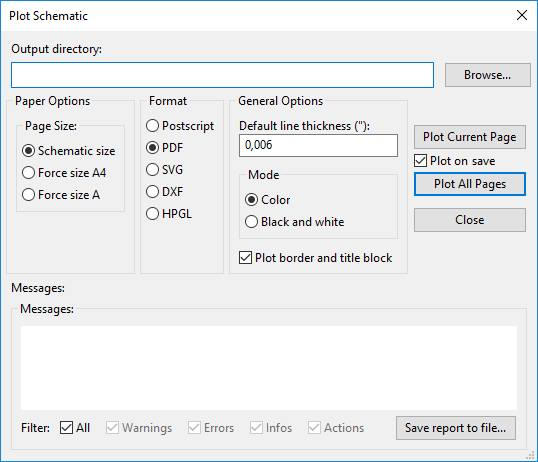
\includegraphics[scale=0.4]{ki_bug_1}
	\caption{Required Mockup}
\end{figure}
\\
The schematic will be plot in PDF format and with scaling the color and the wire width will be taken from the previous setting keeping in mind that they are user defined property i.e. every user might have different requirement of PDF
\section{Bug : Add hotkey for opening context menu in eeschema}
This Bug : \verb!#! 1663595 is also a feature addition in eeschema in which the user wanted to have a shortcut to open the context menu for fast use of the software. The assigned hotkey for this function is \textbf{'D'}. The context menu open a bit below the cousor position.
\vspace{3mm}
\\
Bug Link : \url{https://bugs.launchpad.net/kicad/+bug/1663595}
\\
\\
Patch Link : \url{https://bugs.launchpad.net/kicad/+bug/1663595/+attachment/5159628/+files/0001-Eeschema-Add-shortcut-for-opening-context-menu.patch}
\begin{figure}[h]
	\centering
	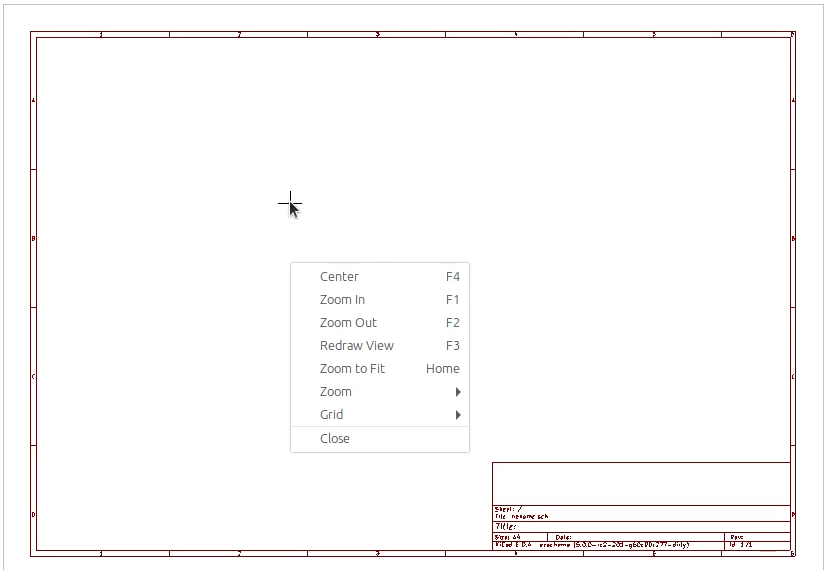
\includegraphics[scale=0.3]{ki_bug_2}
	\caption{Patch Output}
\end{figure}
\\
\textbf{Solution} : Following is the Code Snippet to generate context menu
\begin{verbatim}
case HK_RIGHT_CLICK:
        {
            wxMenu MasterMenu;
            wxPoint pos1 = wxGetMousePosition() , pos2 = GetScreenPosition();
            wxPoint pos = pos1 - pos2;

            if( !OnRightClick( aPosition, &MasterMenu ) )
                return false;

            AddMenuZoomAndGrid( &MasterMenu );

            m_canvas->SetIgnoreMouseEvents(true);
            PopupMenu( &MasterMenu, pos );
            m_canvas->SetIgnoreMouseEvents(false);
        }
\end{verbatim}
\section{Bug : Inconsistent reference field parsing during editor copy}
The bug was posted on Kicad's issue tracker as \href{https://bugs.launchpad.net/kicad/+bug/1748789}{Bug\#1748789} on Launchpad.
\subsection{Description}
``Copy seems to parse the reference such that the prefix is treated as everything up to and including the last non-numeric character. This was a pleasant surprise after the behaviour of KiCAD 4, and should be kept. However, edit seems to parse the reference differently such that the prefix is treated as everything up to but not including the first non-numeric character. These are inconsistent. I would like to have the prefix for both operations being everything up to and including the last non-numeric character."
\subsection{Solution}
From the bug description, it is clear that the required behaviour should parse the last numeric value for the users to be easily able to edit it.
\section{Bug: Ability to open project folder in host operating system}
This is not a bug but a feature request in Kicad. The request is filed as \href{https://bugs.launchpad.net/kicad/+bug/1584977}{Bug\#1584977} on Launchpad.
\subsection{Description}
``Many IDEs and other project-based tools let you open the project's root folder (directory) in the host OS's file manager. I think it would be great if KiCad also had this ability."
\subsection{Solution}
A simple solution this problem is using Cmake to determine the target operating system and using native shell commands to open project directory using default file manager software.\\
\\
To determine the target operating system, following constants can be used

\begin{verbatim}
#if defined(__linux__) || defined(__FreeBSD__)
#define OPEN_FM_CMD_BASE "xdg-open"
#elif defined(__WXMAC__)
#define OPEN_FM_CMD_BASE "open"
#elif defined(_WIN32)
#define OPEN_FM_CMD_BASE "explorer"
#else
#error "Unsupported platform!"
#endif
\end{verbatim}

When the compiler pre-processes above code, a constant \texttt{OPEN\_FM\_CMD\_BASE} will be defined with its value set to appropriate command that can be used to open file explorer on the target operating system.\\
\\
Now, we execute the obtained command with proper arguments to open project directory in operating system's default file explorer
\begin{verbatim}
wxExecute( wxT(OPEN_FM_CMD_BASE " " + project_dir ), wxEXEC_ASYNC, NULL );
\end{verbatim}

\chapter{\textbf{Digital Simulation and Component Parser}}
This Chapter describes about the simulation in ngspice and about the component libraries of Kicad and eSim , similarities and differences between them. Problem description is to find out the reason behind the faliure of ngspice in simulating the digital circuits and some analog circuits in Kicad and to find out if we can use the components of kicad in eSim to increase the eSim library.
\section{Digital Simulation in KiCad}

\begin{wrapfigure}{r}{0.5\textwidth} %this figure will be at the right
	\centering
	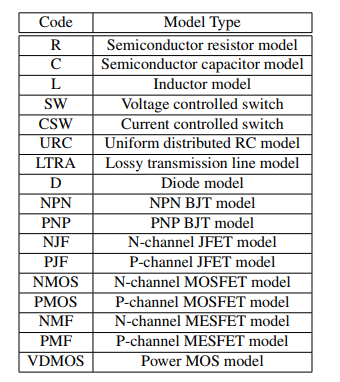
\includegraphics[width=0.5\textwidth]{models}
	\caption{Models in ngSpice}
\end{wrapfigure}

Digital simulation is a problem coming in Kicad on simulating the circuits which works perfectly on eSim. Initially it was suggested that there must be some problem in the way Kicad converts the schematic to its respective generic netlist. On studying he kicad code base it is found that there is some changes in the way kicad identifies the connections from v4 (used in eSim) to v5 (new stable version of kicad). But it is not the only problem, because on changing the connection accordingly the same error pops i.e. \texttt{Error:model not found...} On refering to \href{http://ngspice.sourceforge.net/docs/ngspice-manual.pdf}{ngSpice manual}, it is found that there are some specific components which are identified as models in ngSpice which are shown.
\vspace{5mm}
\\
The problem found out is that for models other than those mention above ngSpice is not able to indetify them, and hence error. For such case ngSpice uses its festiure of subcircuit to make internal circuits for these components. Also among the shown components, basic components like R,C,L are automatically identified by ngSpice but for others i.e. Diodes and Transistors you have to specify them using \texttt{.model} function.
\vspace{5mm}
\\
In eSim, the Kicad to ngSpice Converter uses some of the hardcoded values for these models (stored in \texttt{.xml} format) specified in program and add these lines to the generic spice netlist. Also, in eSim for the models not specified in it, will fail to simulate. So the user have to make subcurcuits for these models in order to make them work.
\vspace{5mm}
\\
Even from the discussion in official \href{https://forum.kicad.info/t/digital-simulation/11072}{KiCad Forum}, it is suggested to make the subcircuits for the components, to make them work.

\section{Parser to increase supported components in eSim}
This section discuss about the suggestion to increase the no of components in eSim from Kicad by making a parser which convert the symbols from Kicad format to eSim format. It is suggested to take help from the \href{https://github.com/FOSSEE/Pspice-Kicad-Converter}{Pspice to Kicad parser} made earlier. On research it is found that the component files of Kicad and eSim are almost same. In fact eSim uses the eeschema software of kicad suit for schematic designing, so the components of kicad can be easily run on eSim, there might be only warning to uses a newer version of eeschema but it does not have any such effect in the running of the prorgam. And even the parser which was made earlier converts files from pspice to kicad which are two completely different softwares (infact competitors), whereas eSim is made on Kicad.
\\ Hence, it is conclude that there is no need to make a parser. In support to our conclusion , few components are added to eSim from Kicad which earlier dont work in eSim. These components include LM741, LM733H.

\subsection{LM741}
\begin{wrapfigure}{l}{0.4\textwidth} %this figure will be at the right
	\centering
	
\includegraphics[width=0.4\textwidth]{lm741}
	\caption{LM741}
\end{wrapfigure}
The LM741 series are general-purpose operational amplifiers which feature improved performance over industry standards like the LM709. They are direct, plug-in replacements for the 709C, LM201, MC1439, and 748 in most applications.
\\
The amplifiers offer many features which make their application nearly foolproof: overload protection on the input and output, no latch-up when the common-mode range is exceeded, as well as freedom from oscillations.
\vspace{5mm}
\\
\begin{flushleft}
\textbf{Subcircuit file of LM741}
\end{flushleft}

\begin{verbatim}
* OPAMP MACRO MODEL (INTREMEDIATE LEVEL)
*                  IN- IN+ VEE    OUT  VCC
.SUBCKT lm741   18 2   1   102 19 81   101 20
Q1	5 1	7	NPN
Q2	6 2	8	NPN
RC1	101	5	95.49
RC2	101	6	95.49
RE1	7	4	43.79
RE2	8	4	43.79
I1	4	102	0.001
* OPEN-LOOP GAIN, FIRST POLE AND SLEW RATE
G1	100 10	6 5 0.0104719
RP1	10	100	9.549MEG
CP1	10	100	0.0016667UF
*OUTPUT STAGE
EOUT	80 100	10 100	1
RO	80	81	100
* INTERNAL REFERENCE
RREF1	101	103	100K
RREF2	103	102	100K
EREF	100 0	103 0 1
R100	100	0	1MEG
.model NPN  NPN(BF=50000)
.ENDS lm741
\end{verbatim}
\vspace{5mm}
\begin{figure}[h]
	\centering
	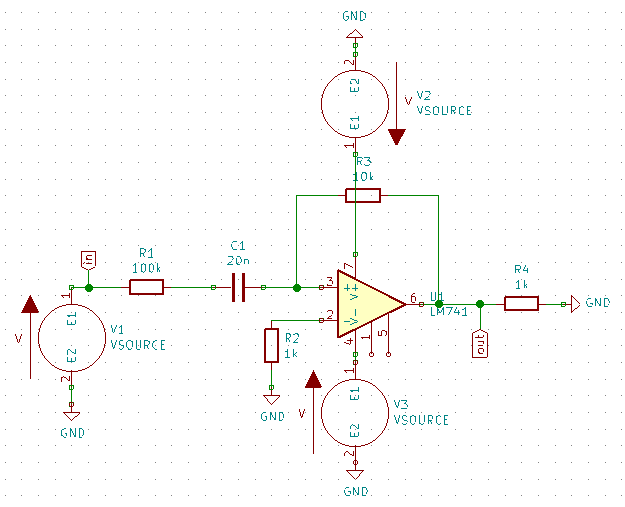
\includegraphics[scale=0.4]{lm741_sch}
	\caption{LM741 - Schematic}
\end{figure}

\vspace{5mm}
\begin{figure}[h]
	\centering
	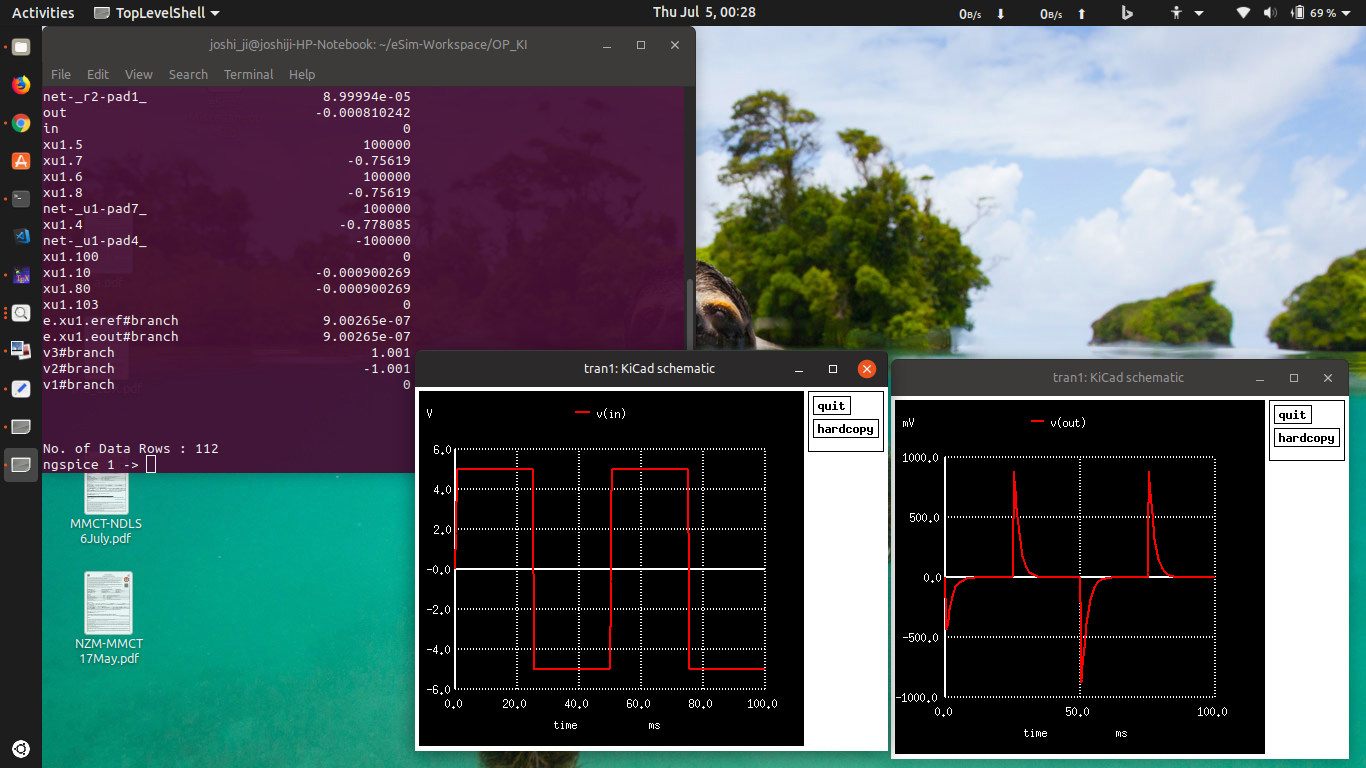
\includegraphics[width=\textwidth]{lm741_sim}
	\caption{LM741 - Simulation Output}
\end{figure}

\subsection{LM733H}
\begin{wrapfigure}{l}{0.4\textwidth} %this figure will be at the right
	\centering
	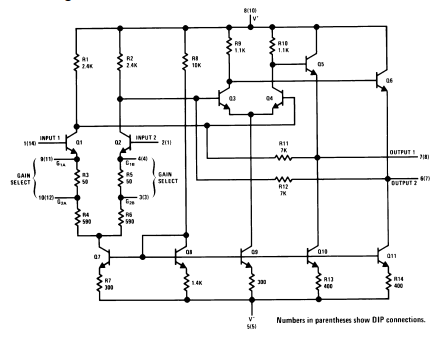
\includegraphics[width=0.4\textwidth]{lm733h_sub}
	\caption{LM733H - Internal Subcircuit}
\end{wrapfigure}
The LM733/LM733C is a two-stage, differential input, differential output, wide-band video amplifier. The use of internal series-shunt feedback gives wide bandwidth with low phase distortion and high gain stability. Emitter-follower outputs provide a high current drive, low impedance capability. Its 120 MHz bandwidth and selectable gains of 10, 100 and 400, without need for frequency compensation, make it a very useful circuit for memory element drivers, pulse amplifiers, and wide band linear gain stages.
\vspace{5mm}
\\
\begin{flushleft}
	\textbf{Subcircuit file of LM733H}
\end{flushleft}

\begin{verbatim}
* Subcircuit LM733H
.subckt LM733H net-_q1-pad2_ net-_q1-pad3_ net-_r2-pad2_ net-_q3-pad3_ 
net-_r6-pad2_ net-_q3-pad2_ net-_r11-pad2_ net-_q10-pad1_ net-_q8-pad1_ 
net-_q10-pad3_ 

r2  net-_q1-pad3_ net-_r2-pad2_ 50
r6  net-_q3-pad3_ net-_r6-pad2_ 50
r3  net-_r2-pad2_ net-_q2-pad1_ 590
r7  net-_r6-pad2_ net-_q2-pad1_ 590
r4  net-_q2-pad3_ net-_r11-pad2_ 300
r9  net-_q4-pad3_ net-_r11-pad2_ 1.4k
r11  net-_q6-pad3_ net-_r11-pad2_ 300
r15  net-_q8-pad3_ net-_r11-pad2_ 400
r16  net-_q11-pad3_ net-_r11-pad2_ 400
r1  net-_q10-pad1_ net-_q1-pad1_ 2.4k
r5  net-_q10-pad1_ net-_q3-pad1_ 2.4k
r10  net-_q10-pad1_ net-_q10-pad2_ 1.1k
r14  net-_q10-pad1_ net-_q7-pad1_ 1.1k
r8  net-_q10-pad1_ net-_q11-pad2_ 10k
r12  net-_q8-pad1_ net-_q1-pad1_ 7k
r13  net-_q10-pad3_ net-_q3-pad1_ 7k
q1  net-_q1-pad1_ net-_q1-pad2_ net-_q1-pad3_ npn
q3  net-_q3-pad1_ net-_q3-pad2_ net-_q3-pad3_ npn
q7  net-_q7-pad1_ net-_q1-pad1_ net-_q5-pad3_ npn
q5  net-_q10-pad2_ net-_q3-pad1_ net-_q5-pad3_ npn
q9  net-_q10-pad1_ net-_q7-pad1_ net-_q8-pad1_ npn
q10  net-_q10-pad1_ net-_q10-pad2_ net-_q10-pad3_ npn
q11  net-_q10-pad3_ net-_q11-pad2_ net-_q11-pad3_ npn
q8  net-_q8-pad1_ net-_q11-pad2_ net-_q8-pad3_ npn
q6  net-_q5-pad3_ net-_q11-pad2_ net-_q6-pad3_ npn
q4  net-_q11-pad2_ net-_q11-pad2_ net-_q4-pad3_ npn
q2  net-_q2-pad1_ net-_q11-pad2_ net-_q2-pad3_ npn

.model npn  NPN( Is=14.34f Xti=3 Eg=1.11 Vaf=74.03 Bf=400 Ne=1.307 
Ise=14.34f Ikf=.2847 Xtb=1.5 Br=6.092 Nc=2 Isc=0 Ikr=0 Rc=1 Cjc=7.306p
Mjc=.3416 Vjc=.75 Fc=.5 Cje=22.01p Mje=.377 Vje=.75 Tr=46.91n Tf=411.1p
Itf=.6 Vtf=1.7 Xtf=3 Rb=10)

.ends LM733H
\end{verbatim}
\vspace{5mm}
\begin{figure}[h]
	\centering
	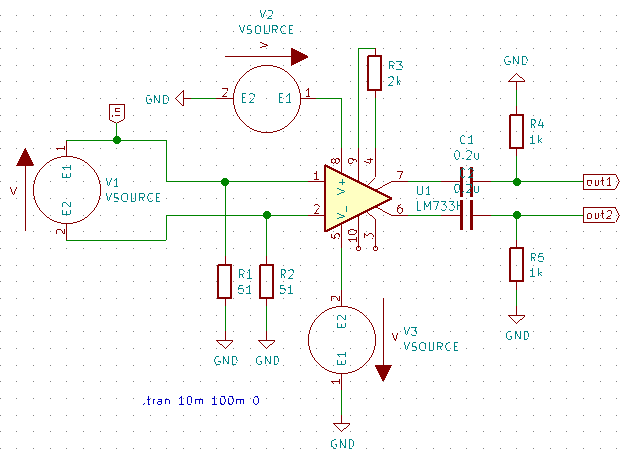
\includegraphics[scale=0.3]{lm733h_sch}
	\caption{LM733H - Schematic}
\end{figure}

\vspace{5mm}
\begin{figure}[h]
	\centering
	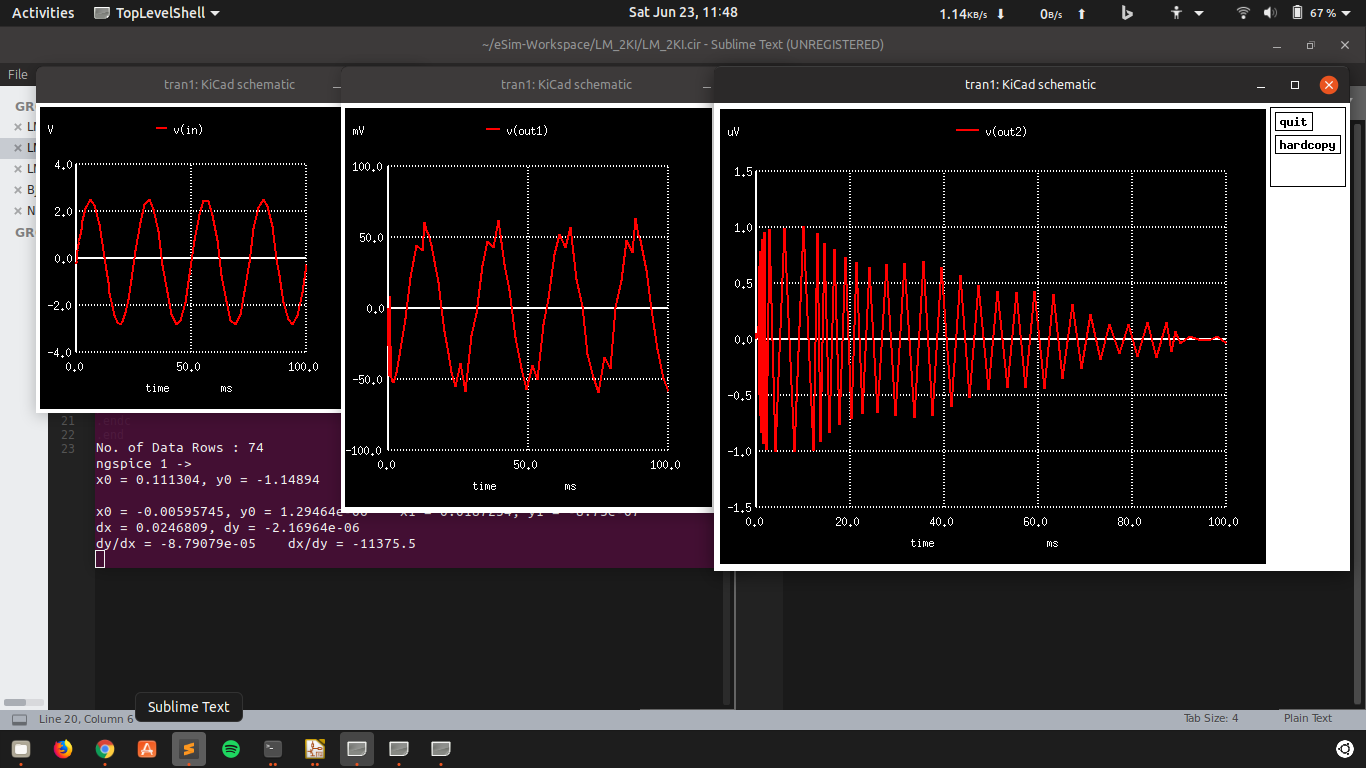
\includegraphics[width=\textwidth]{lm733h_sim}
	\caption{LM733H - Simulation Output}
\end{figure}
\vspace{5mm}
\textbf{\Large Conclusion}
\vspace{5mm}
\\
So after all research and discussion it is concluded that the solution for both digital simulation and parser problem is to make the subcircuit for every components required in the circuit. Also, Kicad being a PCB designing focused software give more preference to the shape of IC and the positioning of pins in the IC rather than what is the internal circuitory of the component. Also the above subcircuits for LM741 and LM733H support the solution. But the problem which arised in this case is the limited no of ports to represent pins of the subcircuit (which is only 8), whose solution is discussed in the next chapter.



\chapter{\textbf{eSim}}
This chapter emphasises on the work done on eSim EDA software, bug fixes, feature additions, and improvement in working.
\section{Increase External Pins for Sub-Circuits}
The problem is inability to make sub-circuits of components having more than 8 pins. It is found that the component \texttt{port} that represents pins of the IC is only 8 so for the ICs having more than 8 pins, their subcircuits cannot be made.
\begin{figure}[h]
	\centering
	
\includegraphics[scale=0.3]{port}
	\caption{eSim\_Miscellaneous - PORT}
\end{figure} 
\\
It is found that the \texttt{port} component, in \texttt{eSim\_Miscellaneous.lib} library file have only option for 8 ports. By increasing them in the \texttt{.lib} file solved the problem.
\\
Now the user can make subcircuits for ICs having upto 26 ports which in turn open the way to increase the number of components in eSim to a large extent.
\\
To test the change subcircuits of LM733H Operational Amplifier was made, whose
sub-circuit, schematic, and simulation is shown in previous chapter.
\vspace{3mm}
\\
Link to commit : \url{https://github.com/FOSSEE/eSim/commit/d48bcd6}
\\
\section{Introduced Rename Project Option}
asasd
\section{Improve handling of unknown components}
asdasd
\section{Introduced workspace functionality in eSim}
The workspace feature in eSim is not functioning properly. There is no option for user the set default workspace, at every start it will ask for the workspace. And also even if we change the workspace, eSim will show the default software to the user and lastly project are not workspace specific i.e. for any workspace projects of all workspaces will be shown.
\\
Solution for this problem involves the addition of \texttt{Default Workspace} option in the workspace dialog box, and adding the ability to change the workspace after esim is started.
\begin{figure}[h]
	\centering
	\begin{minipage}{0.45\textwidth}
		\centering
		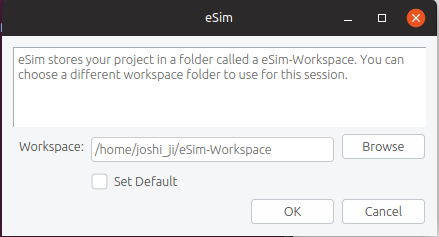
\includegraphics[width=0.9\textwidth]{esim1}
		\caption{Default Workspace Option}
	\end{minipage}\hfill
	\begin{minipage}{0.45\textwidth}
		\centering
		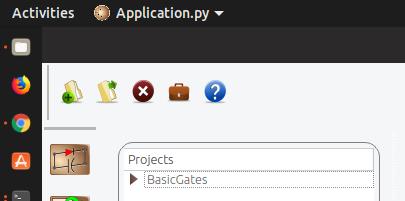
\includegraphics[width=0.9\textwidth]{esim2}
		\caption{Briefcase icon : To change workspace}
	\end{minipage}
\end{figure}
\\
To make projects separated according to workspace, the .projectexplorer file which identifies the projects opened is moved from \texttt{home} folder to the respective workspace folder which make it easier for eSim to classify the projects, and also saves time to unnecessarily process other workspace files.
\vspace{3mm}
\\
Link to commit : \url{https://github.com/FOSSEE/eSim/commit/4347e5d}
\\
\hspace*{28mm} : \url{https://github.com/FOSSEE/eSim/commit/316e3e7}
\\ 
\section{Improve the simulation dependecy problem in new ubuntu version}
This problem appears in newer version of ubuntu (like 18.04). When the user will run simulation for the first time in a project it will not work. Reason being, the function uses ngspice to simulate and then stores it's value in files \texttt{plot\_data\_i.txt} and \texttt{plot\_data\_v.txt} which is used to plot graph in eSim. Ngspice uses \textbf{xterm} terminal emulator to run, which is removed from newer versions of ubuntu. Hence the \texttt{file not found} error will be shown.
\\
This problem is also marked as \verb|#|\texttt{Need Permanent Solution} in the code.
\newpage
\begin{figure}[h]
	\centering
	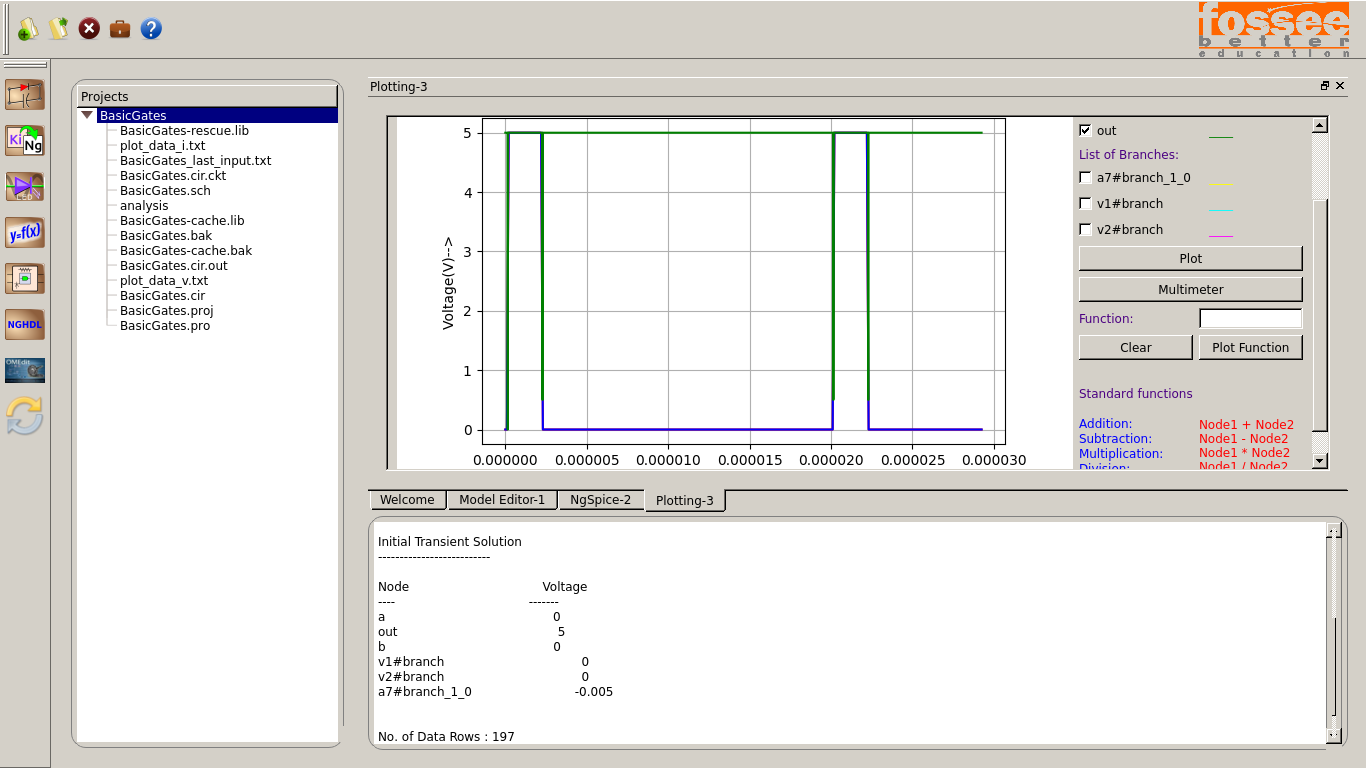
\includegraphics[width=\textwidth]{esim3}
	\caption{New way of simulation and ngspice message}
\end{figure} 
Now all the information related to simulation will be shown in eSim window :
\begin{itemize}
	\itemsep0em
	\item Graph output will come as earlier
	\item Ngspice processing message will come in eSim console window.
	\item User don't need to refer ngspice console.
\end{itemize}
\vspace{3mm}
Link to commit : \url{https://github.com/FOSSEE/eSim/commit/8699521}
\\
\hspace*{28mm} : \url{https://github.com/FOSSEE/eSim/commit/231cd1f}
\\ 

\chapter{\textbf{Standalone Installer for eSim}}
eSim is written in Python 2 and relies on various Python related dependencies to work correctly. In-order for users to be able to install eSim, they had to make sure that several Python related and various other dependencies were installed on their system beforehand. This chapter focuses on overcoming these problems by creating stand-alone executables and native installation packages for eSim.
\section{eSim's dependencies}
\subsection{Python 2.7}
eSim is written in Python and requires Python 2.7 interpreter to run.
\subsection{PyQt4}
eSim uses PyQt4 GUI toolkit for its user interface. It is a Python related dependency for eSim.
\subsection{Matplotlib}
Matplotlib is required for plotting simulations in eSim.  It is also a Python related dependency for eSim.
\subsection{NgSpice}
The Ngspice library is used to provide Spice simulation support in the schematic editor. It is an external dependency.
\subsection{Kicad 4}
eSim uses Kicad 4 for schematic designs of circuits. Kicad 4 is also an external dependency.
\section{PyInstaller}
\href{http://www.pyinstaller.org/}{PyIntaller} is a program that freezes (packages) Python programs into stand-alone executables, under Windows, Linux, Mac OS X, FreeBSD, Solaris and AIX. Its main advantages over similar tools are that PyInstaller works with Python 2.7 and 3.3—3.6, it builds smaller executables thanks to transparent compression, it is fully multi-platform, and use the OS support to load the dynamic libraries, thus ensuring full compatibility.\\
\\
The main goal of PyInstaller is to be compatible with 3rd-party packages out-of-the-box. This means that, with PyInstaller, all the required tricks to make external packages work are already integrated within PyInstaller itself so that there is no user intervention required.\\
\\
With PyInstaller, a stand-alone executable can be created for eSim which wouldn't require any Python-related dependencies to be installed on user's system. With Python related dependencies not required anymore, external dependencies such as Kicad 4 and ngspice can be installed using native installation packages provided by their developers.
\section{Installation Packages}
\subsection{Linux}
Creating Linux installation packages can be lengthy process if not done with the right tools. Since Linux has so many distributions and almost all of them have a different installation package format, creating installation package for each individual distribution can be a tedious part of the development cycle. To avoid the tediousness, several open-source tools like FPM can be used.
\subsubsection{FPM}
\href{https://github.com/jordansissel/fpm}{FPM} is an open-source utility tool written to simplify the process of packaging softwares for various Linux distributions. FPM makes it possible to pack a software's binary into installation package with a single command.\\
\\
With FPM, following installation packages can be generated
\subsubsection*{Debian based Package (.deb)}
FPM can be used to generate a fully functional installation package for Debian based Linux distributions such as Linux Ubuntu, Linux Mint and Debian itself.\\
\\
External dependencies can be passed to FPM with \texttt{--depends} flag. eSim has only two external dependencies, i.e., kicad and ngspice.\\
\\
Following command can be issued to pack eSim into debian package
\begin{verbatim}
    fpm --output-type deb \
    --input-type dir --force \
    --package "dist/$NAME.deb" \
    --name "$NAME" --version "$VERSION" \
    --license "$LICENSE" --vendor "$VENDOR" \
    --description "$DESCRIPTION" --url "$URL" \
    --depends "kicad=4.0" --depends "ngspice" \
    --deb-dist "stable" \
    --deb-no-default-config-files ./dist/esim=/opt \
    esim-linux.desktop-template=/usr/share/applications/esim.desktop \
    esim-launcher.sh=/usr/local/bin/esim
\end{verbatim}
\subsubsection*{Red Hat Linux based Package (.rpm)}
FPM can be used to generate a fully functional installation package for Red Hat based Linux distributions such as Fedora, OpenSUSE and CentOS.\\
\\
External dependencies can be passed to FPM with \texttt{--depends} flag. eSim has only two external dependencies, i.e., kicad and ngspice.\\
\\
Following command can be issued to pack eSim into \texttt{rpm} package
\begin{verbatim}
    fpm --output-type rpm \
    --input-type dir --force \
    --package "dist/$NAME.rpm" \
    --name "$NAME" --version "$VERSION" \
    --license "$LICENSE" --vendor "$VENDOR" \
    --description "$DESCRIPTION" --url "$URL" \
    --depends "kicad-4.0" --depends "ngspice" \
    ./dist/esim=/opt \
    esim-linux.desktop-template=/usr/share/applications/esim.desktop \
    esim-launcher.sh=/usr/local/bin/esim
\end{verbatim}
\subsubsection*{Shell Script Installer}
A generic self extracting shell script based installation package can also be generated using FPM. A shell script based installer should be able to install itself on any Linux based operating system by default.
\subsection{Windows}
Creating a Windows installer requires use of packaging software called InnoSetup.
\\
The setup script \texttt{esim-setup-win.iss} will first add eSim binary files and the kicad and ngspice compressed files to the setup, then registry will be added to run kicad (v4) and ngspice (27) via cmd and finally deletes compressed files. Inno setup compiler is used to change and compile setup script. Final setup will output in \texttt{./dist} directory.


\chapter{\textbf{Conclusion and future work}}
After complete our fellowship, we had been exposed to Open-Source and programmer working life. Throughout our fellowship, we could understand more about the definition of an IT technician and programmer and prepare myself to become a responsible and innovative technician and programmer in future. Along my training period, I realize that observation is a main element to find out the root cause of a problem. Not only for my project but daily activities too. During my project, I cooperate with my colleagues and operators to determine the problems. Moreover, the project indirectly helps me to learn independently, discipline myself, be considerate/patient, self-trust, take initiative and the ability to solve problems. Besides, my communication skills is strengthen as well when communicating with others. During my training period, I have received criticism and advice from engineers and technician when mistakes were made. However, those advices are useful guidance for me to change myself and avoid myself making the same mistakes again. Apart from that, I had also developed my programming skills through various programs that I had done. This also helps sharpen my skills in VB.net 2013 since most of the programs were done with the aid of Visual Studio 2013. In sum, the activities that I had learned during industrial training really are useful for me in future to face challenges in a working environment. Throughout the industrial training, I found that several things are important: 

Critical and Analytical Thinking
To organize our tasks and assignment, we need to analyze our problems and assignment, and to formulate a good solution to the problem. We would have to set contingency plan for the solution, so that we are well prepared for the unforeseeable situations. 

Time Management
As overall technician and programmer are always racing against tight timeline and packed schedule, a proper time management will minimize facing overdue deadlines. An effective time management allows us to do our assignment efficiently and meet our schedules. Scheduling avoids time wastage and allows us to plan ahead, and gaining more as a result. 

Goal Management
Opposing to a Herculean goal seemed to be reachable at first sight, it is better to sub-divide the goals to a few achievable tasks, so that we will be gaining more confidence by accomplishing those tasks. 

Colleague Interactions
In working environment, teamwork is vital in contributing to a strong organization. Teamwork is also essential in reaching the goals of the organization as an entity. Thus, communicating and sharing is much needed in the working environment. Therefore, we should be respecting each other in work, and working together as a team, instead of working alone. This is because working together as a team is easier in reaching our targets, rather than operating individually. 

I would like to once again appreciate everyone who has made my industrial training a superb experience

\end{document}
